% !TEX root = ../main.tex

This section will describe the design decisions, which was made throughout the project. It will start by describing the model of the system with a class diagram, then the architecture will be described. It also introduces some quality attribute scenarios, and android device tactics. And finally it will describe the design of the UI, and the application flows.


\subsection{Class Diagram}
Extending upon the  domain model in figure \ref{fig:dom_diag} a class diagram has been made as shown in figure \ref{fig:class_diagram}. The domain model is in “customer language” while the class model is a Software Engineering discipline. 

\begin{figure}[hbt]
\centering
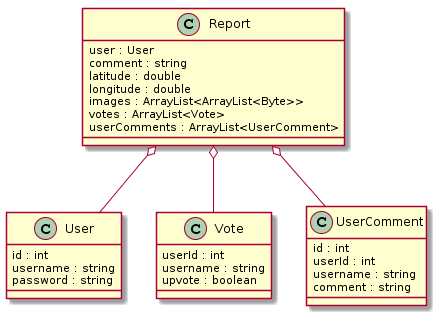
\includegraphics[width=.6\textwidth]{images/Class_model_diagram}
\caption{Class diagram, showing the model of the system.} \label{fig:class_diagram}
\end{figure}

The class diagram in figure \ref{fig:class_diagram} shows the fields of each class and each of their types. The \textit{Report} class aggregates a \textit{User}, a list of \textit{Vote}, and a list of \textit{UserComment} to support the demands for reports having comments and votes as described in the domain model \ref{section:domain_model}. The domain model also describes that a report belongs to a location, this is covered by the fields latitude and longitude. 

%\subsection{Database}
%\todo[inline]{Maybe change the title from Database to Backend and argue that we want Java Spring REST and MySQL. 
%
%...
%
% On second thought. Isn’t this an implementation problem rather than a design problem. idk.}

\subsection{Architecture of prototype diagram}
\subsubsection{Deployment Diagram}
The deployment of the system requires a specific set of computation units. The required units have been mapped the deployment diagram figure \ref{fig:deployment_diagram}.

\begin{figure}[hbt]
\centering
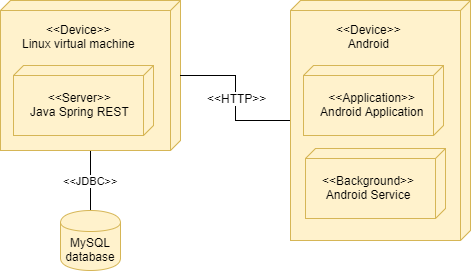
\includegraphics[width=.8\textwidth]{images/Deployment_diagram}
\caption{Deployment diagram of the system.} \label{fig:deployment_diagram}
\end{figure}

Two computational units is the minimum required units to run the system. A Linux virtual machine to host the backend REST service - including a MySQL server to achieve persistence - and at least one Android device. The Android device will act as a client that will consume the REST service provided by the Linux virtual machine. The Android client will be running a continuous background process and will have a frontend app. Both of which will be communicating with the backend through HTTP. The communication protocol between the client and the backend will be HTTP as the server will be a REST service. The communication between the MySQL database and the REST service will be JDBC since this is very well supported in Java.

\subsection{Quality Attribute Scenarios}
This section will introduce some quality attribute scenarios, which will be implemented in order to increase the quality of the system. The quality attribute scenarios in this section focuses on mobile sensing, because of that we only include the quality attributes Energy Efficiency and Resource Adaptability \cite{Kjaergaard2015}.

\subsubsection{Energy Efficiency}
\begin{table}[H]
\centering
\caption{QAS I}
\label{tab:qasI}
\begin{tabularx}{\textwidth}{|l|X|}
\hline
Source of Stimulus & System \\ \hline
Stimulus & Activity recognized as walking, checking if within a geofence \\ \hline
Environment & Not within geofence \\ \hline
Artifact & Client Application \\ \hline
Response & Decrease location service precision. \\ \hline
Response Measure & Maximum 1\% battery drain per hour, caused by this process. \\ \hline
\end{tabularx}
\end{table}

\begin{table}[H]
\centering
\caption{QAS II}
\label{tab:qasII}
\begin{tabularx}{\textwidth}{|l|X|}
\hline
Source of Stimulus & System \\ \hline
Stimulus & Activity recognised as walking, checking if within a geofence \\ \hline
Environment & within geofence \\ \hline
Artifact & Client Application \\ \hline
Response & Increase location service precision. \\ \hline
Response Measure & Maximum 5\% battery drain per hour, caused by this process. \\ \hline
\end{tabularx}
\end{table}

\begin{table}[H]
\centering
\caption{QAS III}
\label{tab:qasIII}
\begin{tabularx}{\textwidth}{|l|X|}
\hline
Source of Stimulus & System \\ \hline
Stimulus & Battery charge below 15 \% \\ \hline
Environment & Normal operations \\ \hline
Artifact & Client application \\ \hline
Response & Disable direct location service, to only receive updates from other services location requests. \\ \hline
Response Measure & Maximum \textless1\% battery drain per hour, caused by this process. \\ \hline
\end{tabularx}
\end{table}

\subsubsection{Resource Adaptability}

\begin{table}[H]
\centering
\caption{QAS IV}
\label{tab:qasIV}
\begin{tabularx}{\textwidth}{|l|X|}
\hline
Source of Stimulus & User \\ \hline
Stimulus & User reports an issue, without client application having permission for location data. \\ \hline
Environment & No location data available. \\ \hline
Artifact & Client application \\ \hline
Response & User is asked to permit location data, or submit a nearby address for reff \\ \hline
Response Measure & increased the reporting time by maximum 2 minutes. \\ \hline
\end{tabularx}
\end{table}

\subsection{Android Device Tactics} \label{sec:tactics}
To address architectural design challenges mentioned above in Quality Attribute Scenarios and to support non-functional requirements, we propose using several architectural, energy efficiency and resource adaptability tactics.

\subsubsection{QAS I and II}
Energy efficiency quality attribute scenario to either increase or decrease location service precision, based on user activity recognition and checking whether user is inside certain geofence radius, can be satisfied by using \textbf{\textit{Event-based}} tactic. This tactic schedules energy consumption of location service when a threshold or raw sensor data indicates an event. The application, continuously checking user activity, will trigger an event when detected activity is recognized as ON FOOT. This, in turn, will start method to check reports proximity to user.  If the application discovers any reports nearby, the location request precision will be increased. If there are no reports, the precision will be lowered.

\subsubsection{QAS III}
Disabling direct location service, to trigger only updates from other applications once the battery charge is below 15\% can be done through setting PRIORITY\_NO\_POWER for setPriority(int) of location request. By setting this, this will greatly limit the functionality of the application, but it will still take advantage of location when available. The tactic used for this is called \textbf{\textit{Sensor Selection}}. It balances quality of service delivered by sensor with energy cost.

\subsubsection{QAS IV}
Resource availability tactic \textbf{\textit{Increase resources}} can be used for our last QAS table. To avoid delivering a degraded quality of service, the tactic increases number of available resources. In our case, we can consider user input as additional resource. When the application fails to deliver location, be it any location or just a correct one, user will have an option to manually submit location data. This could be done by writing down the exact location or referencing nearby address/building/structure for reference.
~\\

Additionally, to have even more efficient application we can consider using tactics outside of our quality attribute scenarios. Continuous location sensing while the service is active consumes a lot of energy. To improve optimization, we can implement \textbf{\textit{Dynamic Duty Cycle}} by setting radius for geofence - in code, by user input through frontend settings, or both. By adjusting this parameter we can lower, or increase if that is needed, the boundary around reports that will trigger method to increase location service precision.
~\\

To continue with the thought that location sensing has high demands on energy, we can use activity recognition service as a trigger for starting location service in chain reaction with tactic named \textbf{\textit{Sensor Replacement}}.
~\\

\textbf{\textit{Communication Selection}} tactic works parallel with Event-based tactic mentioned at the start of this subsection. By reducing the location service precision when the user is not within proximity of any report, the application selects the least energy-consuming communication option to transfer data between requester and provider. The same can be said about the tactic used for QAS III.
~\\

Selecting resources for delivering location updates with the highest quality – in this case we want the latest known user location, helps us deliver augmented service. \textbf{\textit{Resource Selection}} can make use of two methods of Location Request: setInterval(long millis) and setFastestInterval(long millis). By fine-tuning both, we can benefit both from the application's and other applications location updates.


\subsection{User Interface Design} \label{sec:uidesign}
\begin{figure}[H]
\begin{minipage}{.55\textwidth}
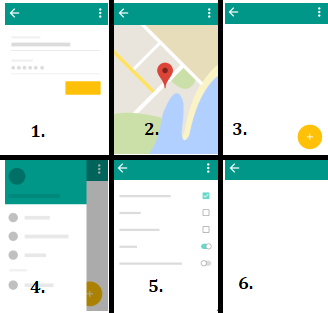
\includegraphics[width=\textwidth]{images/activityDesign}
\caption{Activity Mockups for the application.} \label{fig:activity_design}
\end{minipage}
\hfill
\begin{minipage}{.4\textwidth}
The first prototype of design we will draw inspiration from is figure \ref{fig:activity_design}.
~\\

After user logs in (1), he will be redirected to an activity with Google maps (2). There, he will see his location and reports noted by other users. He can then create his own report (3). The user can navigate with the help of sidebar navigation (4) any time. To adjust the application, user can change settings (5). Finally, some view of user statistics or gamification idea could be displayed in the last activity (6).
\end{minipage}
\end{figure}